\subsection{Punto 4}

A partir del resultado del punto 3, calcular la correlación entre ambas magnitudes.

\subsubsection{Descripción}

Como fuese indicado por la catedra la medida de correlación que calcularemos es el coeficiente de correlación de \textbf{Pearson}.
El coeficiente de correlación de \textbf{Pearson} es una medida de correlación o dependencia entre 2 variables. El mismo varia en los valores ``+1'' y ``-1'' donde una valor ``1'' implica una correlación totalmente positiva, un valor de ``0'' implica que no hay correlación y un valor de ``-1'' implica una correlación totalmente negativa.

\subsubsection{Resultado}

Para la obtención de los datos pedidos modificamos el archivo \textit{runner.py} para que cuando corra la ejecución del ejercicio 3 guarde los datos de ``helpfulness'' y ``length'' en 2 array los cuales luego pasamos a una función que calcula el coeficiente de correlacion de \textbf{Pearson}. A su vez tambien genera el plot de los datos cuando es llamado con el argumento ``--plot''.

\begin{lstlisting}[frame=leftline]
getattr(db,outcoll).aggregate([{"$out" : outcoll}])
coll = getattr(db,outcoll).find()
help = []
length = []
for res in coll:
	print "helpfulness:",
	print res['_id'],
	help.append(float(res['_id']))
	print ", average length:",
	print res['value'] 
	length.append(res['value'])
	print
	print "The Pearson correlation is: %s" % pearson_def(help,length)
		if(args.plot):
		plot(help,length)
\end{lstlisting}

\begin{figure}[H]
  \centering
  \makebox[\textwidth][c]{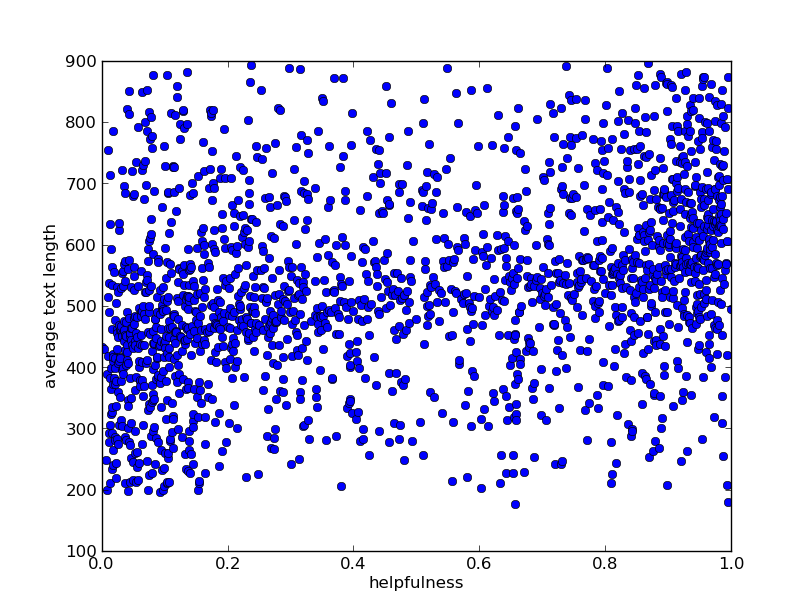
\includegraphics[width=0.70\textwidth]{ej4.png}}%
  \caption{Helpfulness y Length para los datos del ejercicio 3}
  \label{fig41}
\end{figure}

Con los datos del grafico de la figura~\ref{fig41}, el coeficiente de correlación de \textbf{Pearson} obtenido fue de: \textbf{0.322148330724}

\subsubsection{Conclusión}

Dado que el coeficiente de correlación de \textbf{Pearson} es igual a 0.322148330724, podemos concluir que existe cierto grado de correlación positiva entre el puntaje de ``Helpfulness'' y la longitud del texto de la reseña.
Puede observarse en el grafico de la figura~\ref{fig41} que la gran mayoria de los textos tienen una longitud promedio de alrededor de 500 caracteres y son los menos valorados. Se nota tambien cierta tendiencia que al aumentar la longitud del texto aumenta tambien el nivel de valoración.
